\section{Server Backend}
This chapter covers the core component of the iCare Server: The Server Backend. The following subchapters describe the architecture of the server with its individual components and the technologies used to implement communication between the subsystems.
\subsection{The Server architecture}
The following figure \ref{icare-serverarchitecure} shows the general architecture of the backend server and the external systems with which the server communicates at runtime. The focus here lies on the \textit{iCare Server} subsystem, while the other components of the system \textit{iCare Frontend}, \textit{iCare Room HUB}, \textit{iCare Backup System} and \textit{iCare Data} are treated as black boxes. 
\begin{figure}[H]
	\centering
	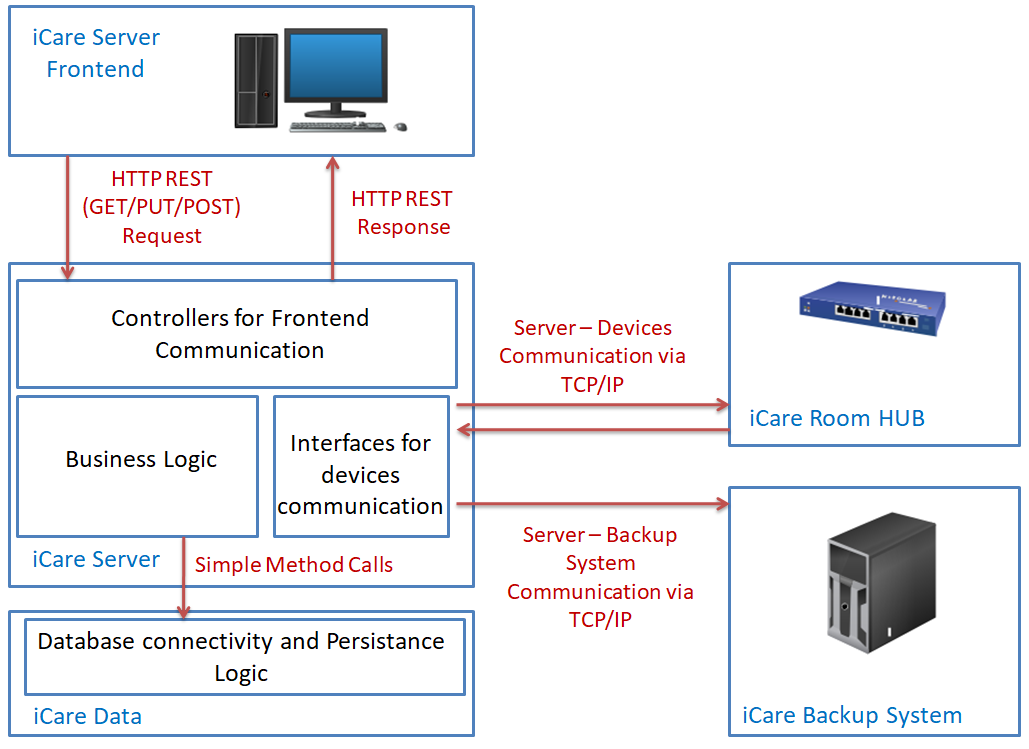
\includegraphics[width =1.0\textwidth]{images/server-architecture.PNG}
	\caption{iCare Server architecture}
	\label{icare-serverarchitecure}
\end{figure}
As can be seen in the picture, the iCare web server has communication interfaces to the other subsystems, which are based on different technologies. The communication between the frontend and the backend is based on Representational State Transfer (REST) web services. The communication with the different devices, which are accessible via a network hub in the individual rooms, works with simple Java sockets. Because the iCare Data module runs on the same system, there is a direct dependency relationship between the iCare Data module and the iCare Server module, enabling the web server to directly access the interfaces of the iCare Data module.
\subsection{Communication between frontend and backend via REST}
As already mentioned, the communication between frontend and backend works via RESTful web services. The web server provides controller classes as access points for the requests of the iCare frontend, which can be reached at the host address of the web server under corresponding extensions. The following address is an example for this kind of access point.
\begin{center}
	\textit{http://www.iCareWeb.de:8080/inhabitant}
\end{center}
The \textit{/inhabitant} access point for example provides a list of all care home residents that carry a wrist band and the corresponding data captured by the wrist band in real time. For example, if the frontend is to display this data in a user interface, a GET request must only be sent to this endpoint at regular intervals. As a response, the frontend receives the current data of all wrist bands packed in a JSON string. The following listing shows one entry in this JSON-String:
\begin{lstlisting}
{
	"id": "a64f3d5c-bade-49f8-b67f-2d5b7d0c55a5",
	"heartRate": 55,
	"name": "Ms. Smith",
	"restrictions": [],
	"healthCheck": {
		"message": "Low heart rate",
		"status": "YELLOW"
	},
	"position": {
		"x": 29,
		"y": 33
	}
}
\end{lstlisting}
How this JSON string is interpreted and displayed lies with the frontend and is not discussed here any further.
\\
The functions for controlling the central heating system can also be called via PUT and POST requests. To do this, a similar JSON string must be packed into the request, which contains the required data. The server then interprets this JSON string and executes the command for the corresponding radiator in the specified room.

\subsection{Communication between Server and Devices/Backup system}
For communication with peripherals, such as sensors or cameras, Java sockets are used, which communicate with the connected devices via a TCP/IP connection. Since all devices determined in the course of the hardware calculation (see chapter\ref{market-analysis}) for this project have the corresponding communication interfaces, it should not be a problem to address them in this way.
\\\\
To ensure the interchangeability of the individual devices, the server uses an interface for communication instead of stationary classes. The creation of the concrete classes for the individual Devices is controlled by the server via a configuration file in which the device-specific settings are noted. For the control of the water or heating system, an additional command interface is introduced, which contains the corresponding changes to the settings of the devices. Figure \ref{icare-interfaces} shows the interfaces used for the communication.
\begin{figure}[H]
	\centering
	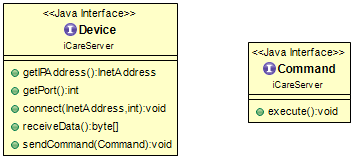
\includegraphics[width =0.65\textwidth]{images/devices.png}
	\caption{iCare Device interfaces}
	\label{icare-interfaces}
\end{figure}
Communication with the backup system is performed in the same way.
\subsection{Business Logic}
The server has several functionalities, which are controlled by a business logic. It receives data at regular intervals from the various devices in the individual rooms, processes and persists them in the database. At the same time, it must transmit images of specific data sets to the backup system so that not all data sets are lost if the server fails. It must also be constantly ready to receive GET, POST and PUT requests from the frontend and process and/or make the corresponding data available. Some of the provided functionalities are presented below.
\subsubsection{Creating Notifications from alerts}
One of the most important functions of the server is to monitor the health status of the care home residents equipped with wristbands and to generate an alarm in the event of an emergency. For this purpose, the server constantly evaluates all data transmitted by the wristbands and generates a notification with the corresponding severity if a resident's state of health shows anomalies or if he enters an area that is forbidden for him. The notification contains all important data. This also includes the room in which the alarm was triggered. The following figure shows a representation of this use case:
\begin{figure}[H]
	\centering
	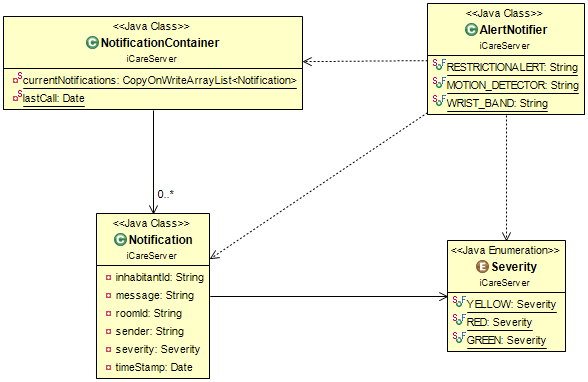
\includegraphics[width =0.8\textwidth]{images/notification.png}
	\caption{iCare Alarm Notifications}
	\label{icare-notification}
\end{figure}
These notifications are stored in a container. Since the frontend constantly queries all current notifications from the server, it is ensured that the alarm is perceived by the staff and help can be sent quickly.
\subsubsection{Monitoring the energy and water consumption}
Another important task of the server is to monitor the energy and water consumption of the care home using the central heating system and the connected water meters in the individual rooms. The collected data is processed using the HouseState singleton, which tracks the current consumption of the building. HouseState objects are then generated and forwarded to the database for persistence using a time stamp. These objects are also used by the controller to provide the data for display in the frontend.
\begin{figure}[H]
	\centering
	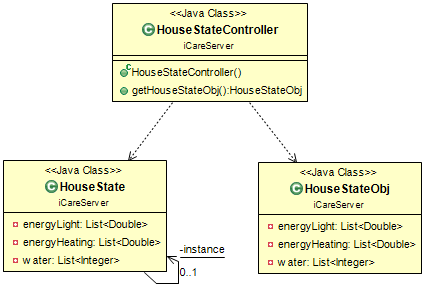
\includegraphics[width =0.8\textwidth]{images/houseState.png}
	\caption{iCare Energy and Water Consumption}
	\label{icare-houseState}
\end{figure}
There are other tasks that the server performs in parallel to the two functions demonstrated. However, these are no longer presented here, as they would go beyond the scope of this document.
\subsection{Connection to ICare Data}
The ICare Data Module is operated on the same machine as the server itself. It is a separate module that establishes the connection to the database and thus persists the data. Since the server is directly dependent on this module, it accesses the module's functionality via simple method calls. The iCare Data Module is described in more detail in Chapter \ref{label}.